\subsection{Mặt phẳng hai chiều và hệ tọa độ vuông góc}

\begin{figure}[h]
   \centering
   \begin{minipage}[b]{0.48\textwidth}
      \centering
      \begin{tikzpicture}
         \draw[->] (-2,0) -- (2,0);
         \draw[->] (0,-2) -- (0,2);
         \node[right] at (2,0) {Trục hoành};
         \node[above] at (0,2) {Trục tung};
         \filldraw (0, 0) circle (1.5pt);
         \node[below left] at (0, 0) {$O(0; 0)$};

         \node at (1,1) {$\boxed{\text{I}}$};
         \node at (-1,1) {$\boxed{\text{II}}$};
         \node at (1,-1) {$\boxed{\text{IV}}$};
         \node at (-1,-1) {$\boxed{\text{III}}$};

         \draw (1,0) -- (1,-0.08) node[below] {$x_P$};
         \draw (0,1.5) -- (-0.08,1.5) node[left] {$y_P$};

         \filldraw (1, 1.5) circle (1.5pt);
         \node[above right] at (1, 1.5) {$P(x_P; y_P)$};

         \draw[dashed] (1, 1.5) -- (1, 0);
         \draw[dashed] (1, 1.5) -- (0, 1.5);
      \end{tikzpicture}
      \caption{Hệ tọa độ vuông góc}
      \label{fig:toa do vuong goc}
   \end{minipage}
   \hfill
   \begin{minipage}[b]{0.48\textwidth}
      \centering
      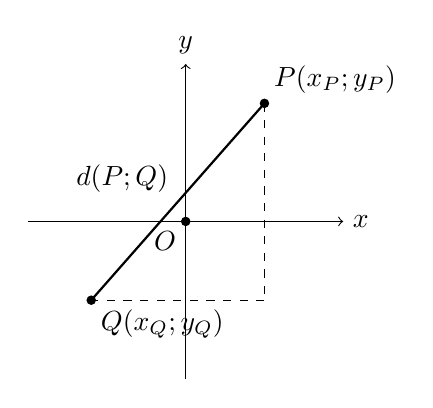
\begin{tikzpicture}
         \draw[->] (-2,0) -- (2,0);
         \draw[->] (0,-2) -- (0,2);
         \node[right] at (2,0) {$x$};
         \node[above] at (0,2) {$y$};
         \filldraw (0, 0) circle (1.5pt);
         \node[below left] at (0, 0) {$O$};

         \pgfmathsetmacro{\xP}{1}
         \pgfmathsetmacro{\yP}{1.5}
         \pgfmathsetmacro{\xQ}{-1.2}
         \pgfmathsetmacro{\yQ}{-1}

         \filldraw (\xP, \yP) circle (1.5pt);
         \node[above right] at (\xP, \yP) {$P(x_P; y_P)$};

         \filldraw (\xQ, \yQ) circle (1.5pt);
         \node[below right] at (\xQ, \yQ) {$Q(x_Q; y_Q)$};

         \draw[thick] (\xP, \yP) -- (\xQ, \yQ);
         \draw[dashed] (\xP, \yP) -- (\xP, \yQ);
         \draw[dashed] (\xP, \yQ) -- (\xQ, \yQ);

         \node[above left] at ({(\xP+\xQ)/2}, {(\yP+\yQ)/2}) {$d(P;Q)$};
      \end{tikzpicture}
      \caption{Khoảng cách giữa hai điểm}
      \label{fig:khoang cach 2d}
   \end{minipage}
\end{figure}


Mở rộng lên mặt phẳng hai chiều, nếu chúng ta đặt hai trục vuông góc với nhau và giao nhau tại gốc $O(0)$ của mỗi trục, khi đó, chúng ta có thể xác định vị trị của điểm trên mặt phẳng chứa hai trục theo biểu diễn đại số bằng cách dóng điểm đó lên trục mà sau này được gọi là \emph{tọa độ}. Đây được gọi là \emph{hệ tọa độ vuông góc} (hay \emph{hệ tọa độ Đề-các}\footnote{René Descartes (1596-1650)}). Như ở hình \ref{fig:toa do vuong goc}, trục nằm ngang được gọi là \emph{trục hoành}, trục dọc được gọi là \emph{trục tung}. Tùy trong từng trường hợp, vị trí và hướng chỉ của các trục có thể thay đổi. Với mỗi điểm, vị trí khi dóng điểm đó vào trục hoành gọi là \emph{hoành độ}, vào trục tung gọi là \emph{tung độ}. Tiếp tục lấy ví dụ từ hình \ref{fig:toa do vuong goc}, điểm $P$ có tọa độ là $(x_P;y_P)$ và được kí hiệu là $P(x_P;y_P)$. Thêm vào đó, hai trục chia mặt phẳng thành bốn góc phần tư, từ góc phần tư thứ I đến góc phần tư thứ IV bao gồm các điểm thỏa mãn tính chất sau:
\begin{itemize}
   \item Góc phần tư thứ I: $x>0$, $y>0$;
   \item Góc phần tư thứ II: $x<0$, $y>0$;
   \item Góc phần tư thứ III: $x<0$, $y<0$;
   \item Góc phần tư thứ IV: $x>0$, $y<0$.
\end{itemize}
Về mặt hình học, khi tọa độ được vẽ thông thường, góc phần tư thứ I nằm ở vị trí trên cùng bên phải, và các góc phần tư còn lại lần lượt được đánh số theo ngược chiều kim đồng hồ. Khi tọa độ bị thay đổi thì vị trí các góc phần tư cũng thay đổi theo, nhưng vẫn thỏa mãn điều kiện đại số ở trên. Các điểm trên trục không xác định thuộc bất cứ góc phần tư nào.

Giống như trên trục một chiều, khi có hai điểm trên mặt phẳng thì chúng ta có thể tính khoảng cách giữa chúng. Một cách chi tiết, cho hai điểm $P(x_P;y_P)$ và $Q(x_Q;y_Q)$, theo định lí Pi-ta-go, khoảng cách giữa hai điểm đó là $$d(P;Q)=\sqrt{(x_P-x_Q)^2+(y_P-y_Q)^2}.$$

\exercise[ex:0.2] Biểu diễn các điểm sau trên hệ tọa độ vuông góc: $A(2;3)$, $B(-1;2)$, $C(-3;0)$, $D(0;4)$, $P(12t;-3t)$, $Q(20t;12t)$ (với $t \in \mathbb{R}$). Xác định góc phần tư hoặc trục tọa độ của mỗi điểm. Sau đó, tính khoảng cách giữa những cặp điểm sau: $A$ và $B$, $C$ và $D$, $P$ và $Q$.

\solution[ex:0.2]

\begin{figure}[h]
   \centering
   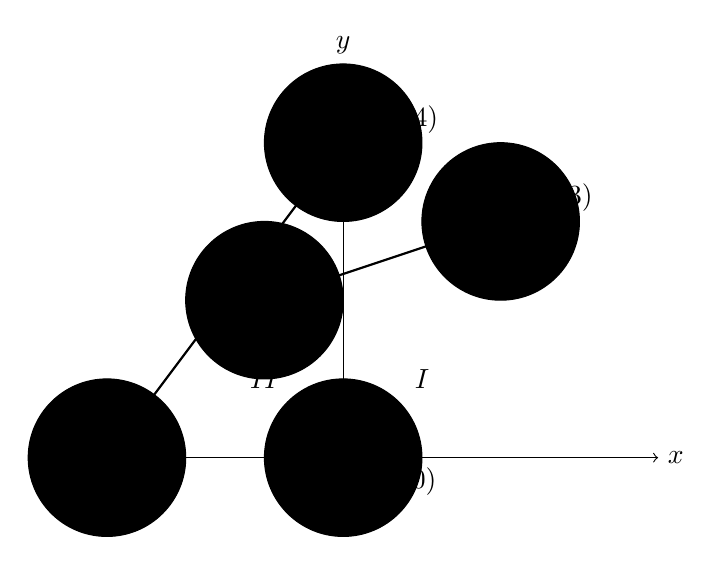
\begin{tikzpicture}
      \draw[->] (-4,0) -- (4,0);
      \draw[->] (0,-1) -- (0,5);
      \node[right] at (4,0) {$x$};
      \node[above] at (0,5) {$y$};
      \filldraw (0, 0) circle (\pointSize) node[below right] {$O(0;0)$};
      \filldraw (2, 3) circle (\pointSize) node[above right] {$A(2;3)$};
      \filldraw (-1, 2) circle (\pointSize) node[below] {$B(-1;2)$};
      \filldraw (-3, 0) circle (\pointSize) node[below] {$C(-3;0)$};
      \filldraw (0, 4) circle (\pointSize) node[above right] {$D(0;4)$};
      \draw[thick] (2, 3) -- (-1, 2);
      \draw[thick] (-3, 0) -- (0, 4);

      \node at (1,1) {$\boxed{\text{I}}$};
      \node at (-1,1) {$\boxed{\text{II}}$};
   \end{tikzpicture}
   \caption{Biểu diễn các điểm $A$, $B$, $C$, $D$ trong bài \ref{ex:0.2}}
   \label{fig:toa do vuong goc bai tap}
\end{figure}

Các góc phần tư hay trục số mà các điểm thuộc về có thể được xác định như hình \ref{fig:toa do vuong goc bai tap}. Theo một cách khác, về mặt đại số, có:
\begin{itemize}
   \item $A(2;3)$: $x>0$, $y>0 \implies A$ thuộc góc phần tư thứ I;
   \item $B(-1;2)$: $x<0$, $y>0 \implies B$ thuộc góc phần tư thứ II;
   \item $C(-3;0)$: $x<0$, $y=0 \implies C$ thuộc trục hoành;
   \item $D(0;4)$: $x=0$, $y>0 \implies D$ thuộc trục tung.
\end{itemize}

\begin{figure}[h]
   \centering
   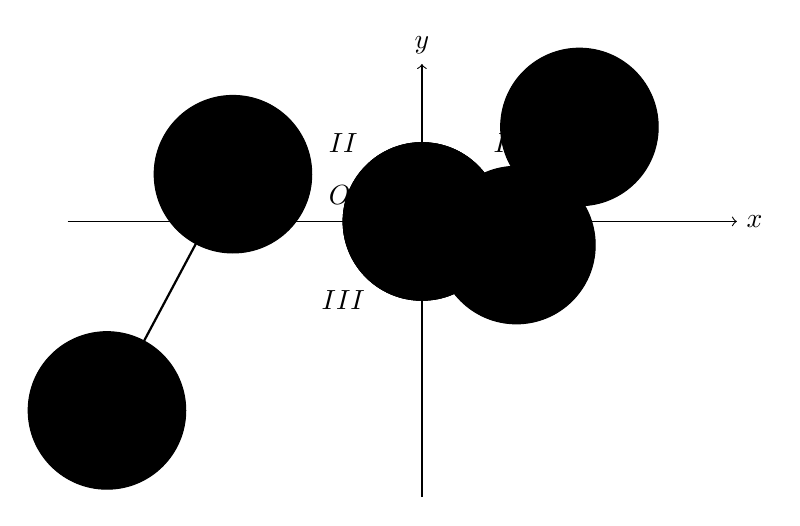
\begin{tikzpicture}
      \draw[->] (-4.5,0) -- (4,0);
      \draw[->] (0,-3.5) -- (0,2);
      \node[right] at (4,0) {$x$};
      \node[above] at (0,2) {$y$};
      \filldraw (0, 0) circle (\pointSize) node[above left] {$O(0;0)$};
      \filldraw (0, 0) circle (\pointSize) node[below right] {$P_{t=0}$};
      \filldraw (0, 0) circle (\pointSize) node[above right] {$Q_{t=0}$};

      \node at (1,1) {$\boxed{\text{I}}$};
      \node at (-1,-1) {$\boxed{\text{III}}$};
      \node at (-1,1) {$\boxed{\text{II}}$};
      \node at (1,-1) {$\boxed{\text{IV}}$};
      \pgfmathsetmacro{\t}{0.1}
      \filldraw ({12*\t}, {-3*\t}) circle (\pointSize) node[below right] {$P_{t_+}$};
      \filldraw ({20*\t}, {12*\t}) circle (\pointSize) node[above right] {$Q_{t_+}$};
      \draw[thick] ({12*\t}, {-3*\t}) -- ({20*\t}, {12*\t});
      \filldraw ({12*(-\t-0.1)}, {-3*(-\t-0.1)}) circle (\pointSize) node[below right] {$P_{t_-}$};
      \filldraw ({20*(-\t-0.1)}, {12*(-\t-0.1)}) circle (\pointSize) node[below left] {$Q_{t_-}$};
      \draw[thick] ({12*(-\t-0.1)}, {-3*(-\t-0.1)}) -- ({20*(-\t-0.1)}, {12*(-\t-0.1)});
   \end{tikzpicture}
   \caption{Biểu diễn các điểm $P$, $Q$ trong bài \ref{ex:0.2}} theo các trường hợp
   \label{fig:toa do vuong goc PQ}
\end{figure}

Để xác định được vị trí của hai điểm $P$ và $Q$, cần phải xét giá trị của $t$. Nếu $t$ dương, thì $P$ và $Q$ sẽ có tọa độ là $P_{t_+}(12t;-3t)$ và $Q_{t_+}(20t;12t)$ với $x_{P_{t_+}}>0$, $y_{P_{t_+}}<0$ và $x_{Q_{t_+}}>0$, $y_{Q_{t_+}}>0$. Khi này, chúng ta có thể kết luận rằng $P$ thuộc góc phần tư thứ IV và $Q$ thuộc góc phần tư thứ I. Ngược lại, nếu $t$ âm, thì $P$ và $Q$ sẽ có tọa độ là $P_{t_-}(12t;-3t)$ và $Q_{t_-}(20t;12t)$ với $x_{P_{t_-}}<0$, $y_{P_{t_-}}>0$ và $x_{Q_{t_-}}<0$, $y_{Q_{t_-}}<0$. Khi này, $P$ thuộc góc phần tư thứ II và $Q$ thuộc góc phần tư thứ III. Cuối cùng, nếu $t=0$, thì cả hai điểm đều có tọa độ là $(0;0)$, tức là chúng trùng với gốc tọa độ.

Khoảng cách giữa những cặp điểm được yêu cầu là:
\begin{itemize}
   \item $d(A;B) = \sqrt{\left(2-(-1)\right)^2+\left(3-2\right)^2} = \sqrt{10} \approx 3{,}1623$;
   \item $d(C;D) = \sqrt{\left(-3-0\right)^2+\left(0-4\right)^2} = 5$;
   \item $d(P;Q) = \sqrt{\left(12t-20t\right)^2+\left(-3t-12t\right)^2} = 13|t|$.
\end{itemize}
